\section{AIT and Kolmogorov complexity}
%%%%%%%%%%%%%%%%%%%%%%%%%%%%%%%%%%%%%%%%%%%%%%%%%%%%%%%%%%%%%%%%%%%%%%
\begin{frame}[label=intro3]{Kolmogorov complexity ($\Ko$)}
 Agents are physical dynamical systems calculating (effectively computable) functions.   This leads us to analyze agents from the standpoint of computation theory.
 \begin{alertblock}{\textit{Warning}: Computation is a mathematical concept (Turing machine)}
The use of computational framework in KT should not be construed to mean that the brain is literally a physical von Neumann computer (such as a laptop).
\end{alertblock}\vfill 
 
A computational perspective  leads us directly into AIT and its central concept: 


\begin{definition}[\textbf{Kolmogorov complexity}  of a dataset ($\Ko$)]
The length of the shortest program capable of generating  the dataset \citep{Kolomgorov1965}.  
\end{definition}
\end{frame}


%%%%%%%%%%%%%%%%%%%%%%%%%%%%%%%%%%%%%%%%%%%%%%%%%%%%%%%%%%%%%%%%%%%%%%
% \begin{frame}[label=intro3]{Kolmogorov complexity ($\Ko$) II}
%  \begin{center}%\includegraphics[height=1.2cm]{COPL}%
%   %\hspace{2cm}
%   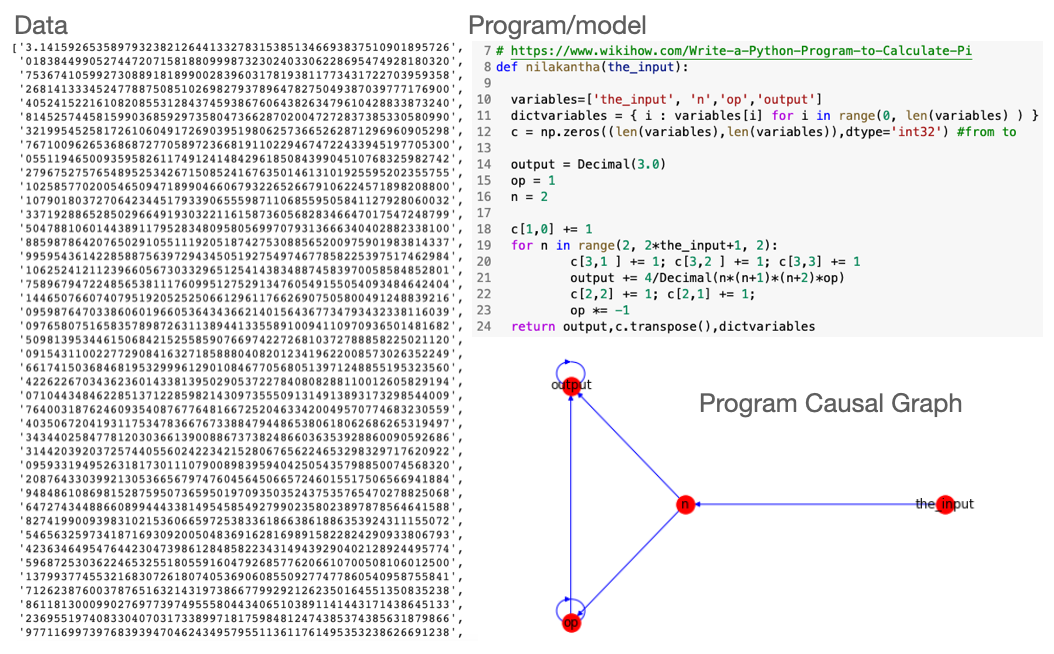
\includegraphics[height=7.2cm]{img/pi.png}
%   \end{center}
% \end{frame}

%%%%%%%%%%%%%%%%%%%%%%%%%%%%%%%%%%%%%%%%%%%%%%%%%%%%%%%%%%%%%%%%%%%%%%
% \begin{frame}[label=intro3]{Mutual algorithmic information ($\mathcal M$)}
% With 
% \K at hand, we can define an algorithmic version of mutual information we will also need: \vfill

% \begin{definition}[Mutual algorithmic information complexity  $\mathcal M$]
% The {\em mutual algorithmic information  $\mathcal M(x:y)$ between two strings $x$ and $y$, is given by\citep{Li:1997aa, Grunwald:2004aa}   }
% $$
% \mathcal M(x \!:\!y) = \Ko(x) +\Ko(y)- \Ko(x,y)
% $$
% %where $\Ko(y|x)$ is the complexity of the string $y$ if the computer has access to $x$ 
% \end{definition}
% \end{frame}

%%%%%%%%%%%%%%%%%%%%%%%%%%%%%%%%%%%%%%%%%%%%%%%%%%%%%%%%%%%%%%%%%%%%%%
% \begin{frame}[label=ladila]{Hierarchy class \citep{Fitch2014}}
% Not all programming languages are equal. Recurrence is needed for Turing completeness, for example. 
%  \begin{center}%\includegraphics[height=1.2cm]{COPL}%
%   %\hspace{2cm}
%   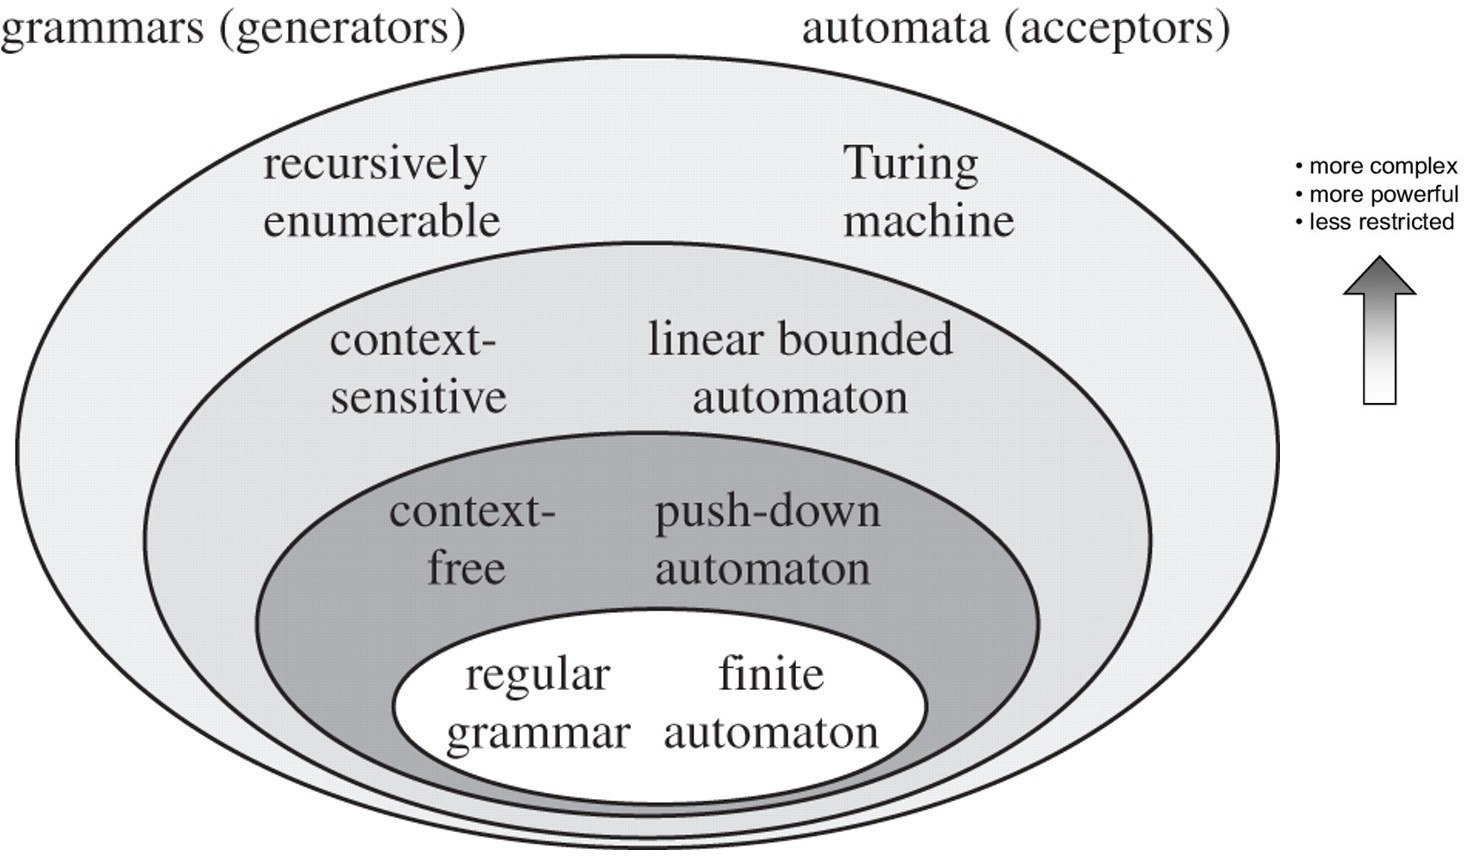
\includegraphics[height=5.5cm]{img/chomsky.jpg}
%   \end{center}
% \end{frame}

%%%%%%%%%%%%%%%%%%%%%%%%%%%%%%%%%%%%%%%%%%%%%%%%%%%%%%%%%%%%%%%%%%%%%%
\begin{frame}[label=ladila]{What is a model? Link with Compression and $\Ko$}
The notion of {\em model} is central in KT and other theories of consciousness. \vfill

 %With AIT as a basis, we can now define what a  model is and an optimal model. \vfill 
 
 \begin{definition}[\textbf{Model} of a dataset]
 A program that generates the dataset. 
 \end{definition} \vfill
%Models may differ in two ways: they may implement different functions, or they may implement the same function in different ways. Both aspects matter here.  We focus on those that implement the right functions succinctly. \vfill 
 
\begin{definition}[\textbf{Optimal model} of a dataset (defines $\Ko$ of the dataset)]
The shortest program that generates (or, equivalently, compresses) the dataset.
\end{definition}\vfill
In practice, agents don't have access to the optimal model! They make do with approximations. (In fact $\Ko$ is uncomputable.)
\end{frame}


%%%%%%%%%%%%%%%%%%%%%%%%%%%%%%%%%%%%%%%%%%%%%%%%%%%%%%%%%%%%%%%%%%%%%%
% \begin{frame}[label=ladila]{Model II}

% An {\bf optimal model needs to capture and exploit all the structure in the dataset}---and nothing else. In some sense, the {\em structure of the model can be described by the group of symmetries of the dataset}  \citep{Ruffini:2016ad}. 
%  \begin{center}%\includegraphics[height=1.2cm]{COPL}%
%   %\hspace{2cm}
%   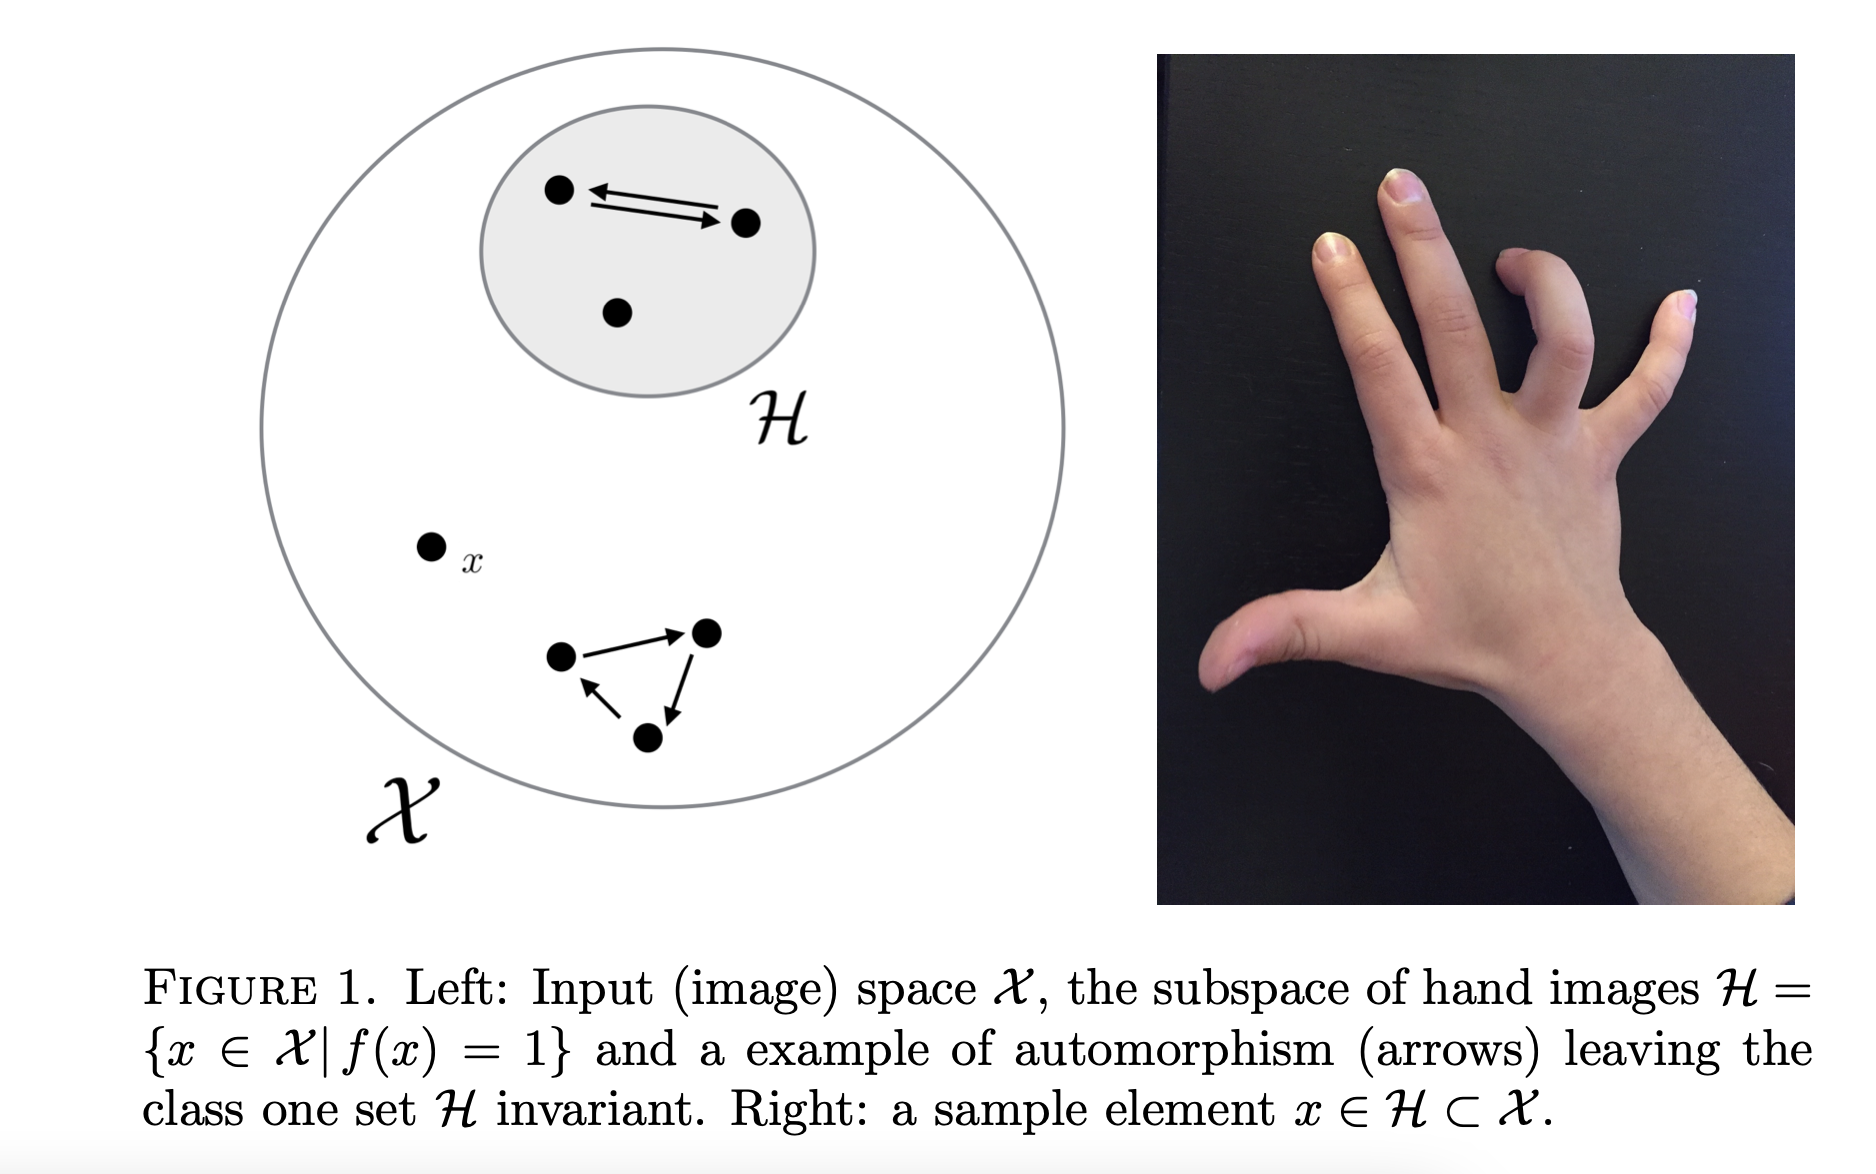
\includegraphics[height=4cm]{img/hand2.png}
%   \end{center}
  
% Suppose we are given a stack of images of a hand, e.g., from the frames of a movie of a moving hand created using a generating function,
% $y = f(\theta)$, where $y$ is the image in a frame and $\theta$ a parametrization of the hand image and view.
% \end{frame}

% \begin{frame}[label=ladila]{Model III}
%  \begin{center}%\includegraphics[height=1.2cm]{COPL}%
%   %\hspace{2cm}
%   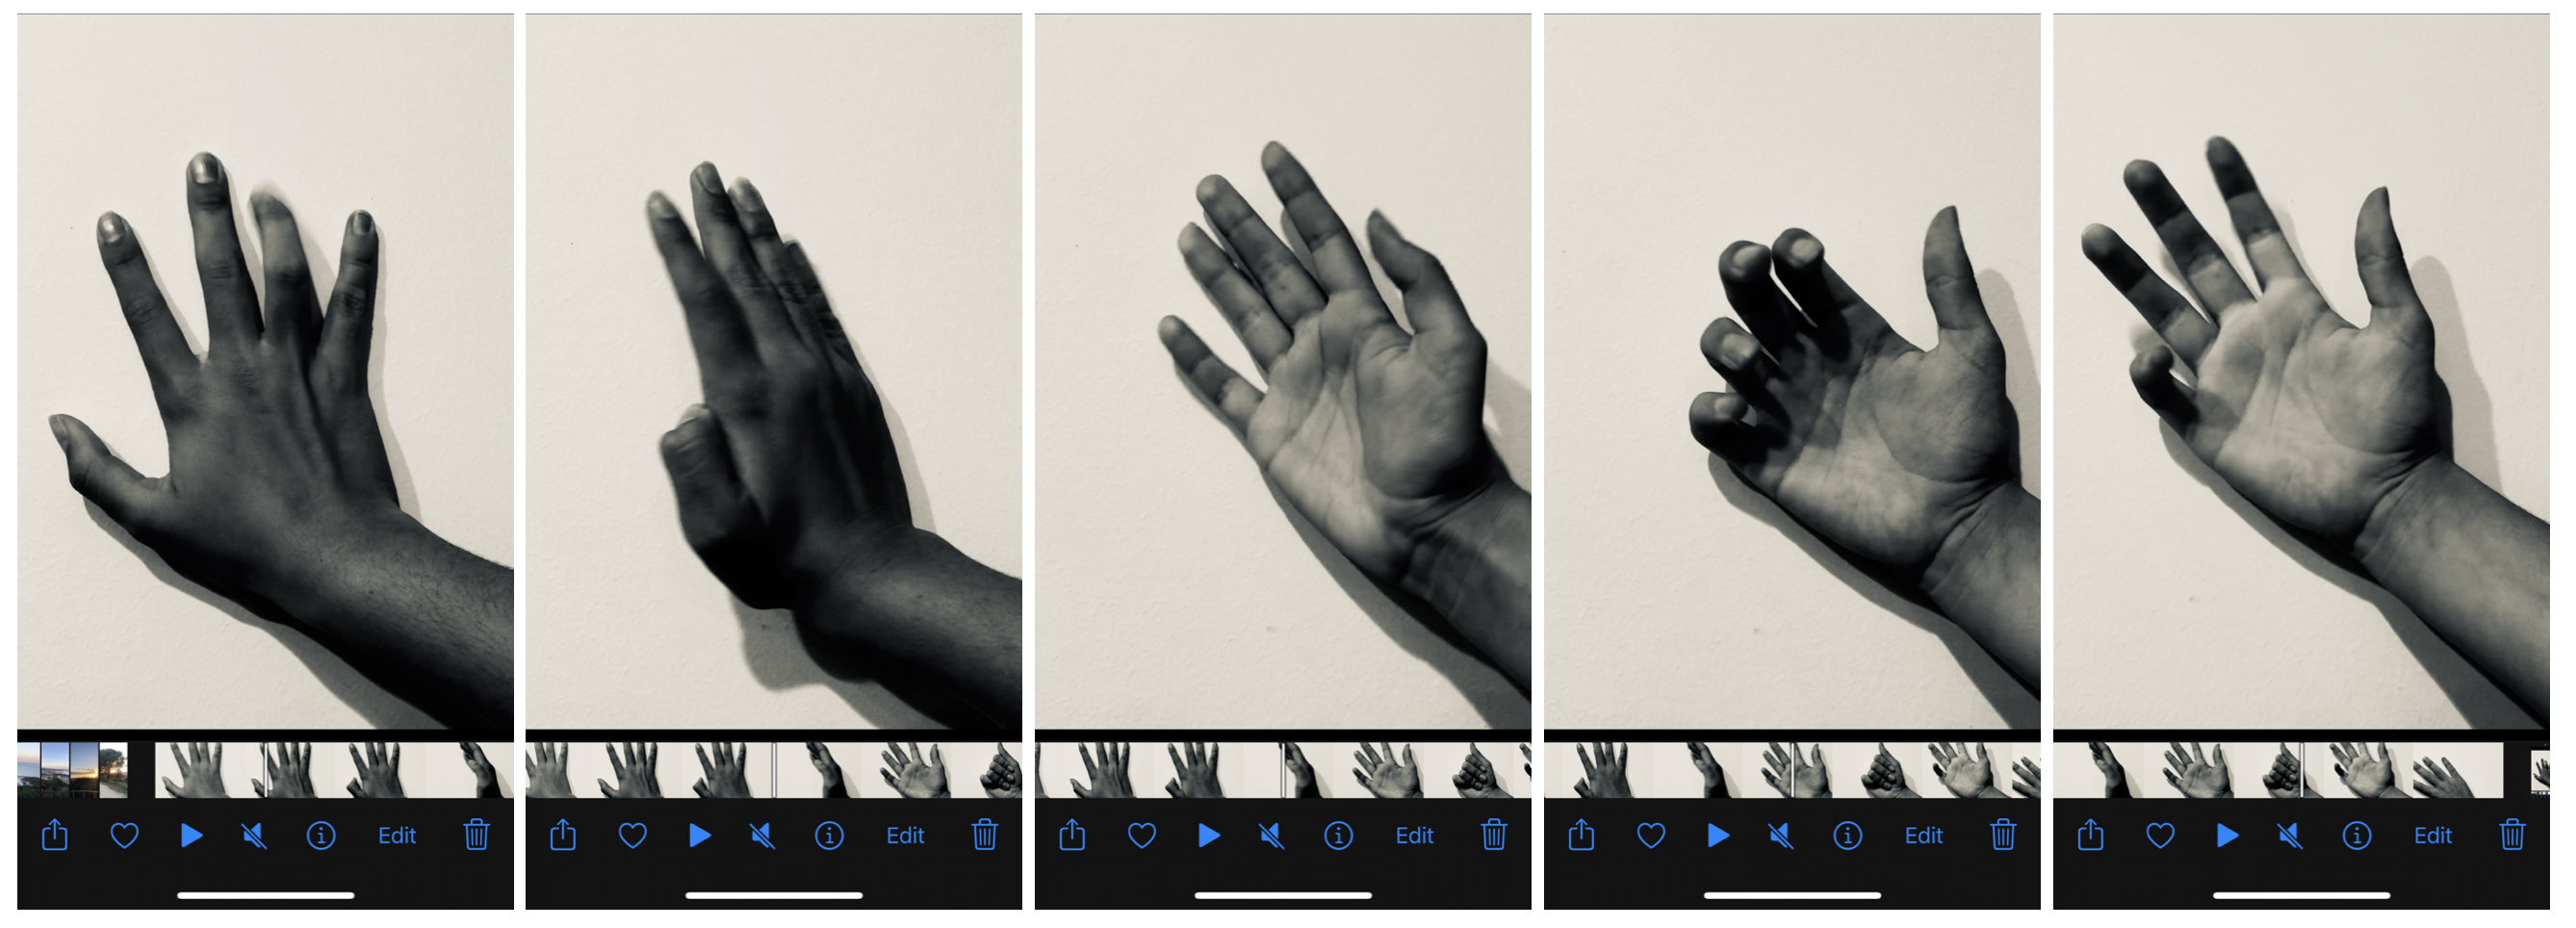
\includegraphics[height=5cm]{img/hands.png}
%   \end{center}
%   The structure of the dataset is encapsulated by the minimal program that encodes the function $y=f(x)$---the {\em invariant} object.  %The {\bf symmetries} of the dataset are parametrized by $\theta$, and they are symmetries in the sense that if $\theta\rightarrow \theta'$ and $y\rightarrow y'$, then the equation $y'-f(\theta') =0 $ holds true.
% \end{frame}



%%%%%%%%%%%%%%%%%%%%%%%%%%%%%%%%%%%%%%%%%%%%%%%%%%%%%%%%%%%%%%%%%%%%%%
\begin{frame}[label=ladila]{Why are succinct models (short programs) useful?}

Occam’s Razor\cite{Ruffini:2007aa,Ruffini:2009aa,Ruffini2017}: {\em
one should not increase, beyond what is necessary, the number of entities required to explain anything.}  \vfill

Ok, but \textbf{why}? Potential answers:\vfill

a) \textbf{The universe is simple}. Simple rules can create apparent complexity. E.g., simple data generators are more likely if the universe rules are drawn from a random algorithmic bingo (Solomonoff's prior).\vfill


 
b) \textbf{Natural selection}: selects agents that coarse grain the world in a way that can be modeled simply. This motivates a definition of \textbf{Emergence}.

 
\end{frame}

\begin{frame}[label=emergence]{From the algorithmic agent to emergence}

To survive, agents must find patterns and operate at some coarse-graining level.

\begin{definition}[Emergence]
  %\textbf{Emergence} is observed by agents when their coarse-graining of a complex system transforms data that appears incompressible (with high apparent Kolmogorov complexity and high entropy) into a new system that retains non-trivial structure (high entropy) and can be compressed by a simpler, lower-complexity model \cite{ruffiniNavigatingComplexityHow2024}.  
  \textbf{Emergence} occurs when coarse-graining transforms data that appears incompressible (with high apparent Kolmogorov complexity and high entropy) into data that can be usefully compressed (modeled)\cite{ruffiniNavigatingComplexityHow2024}.
\end{definition}

\begin{center} 
  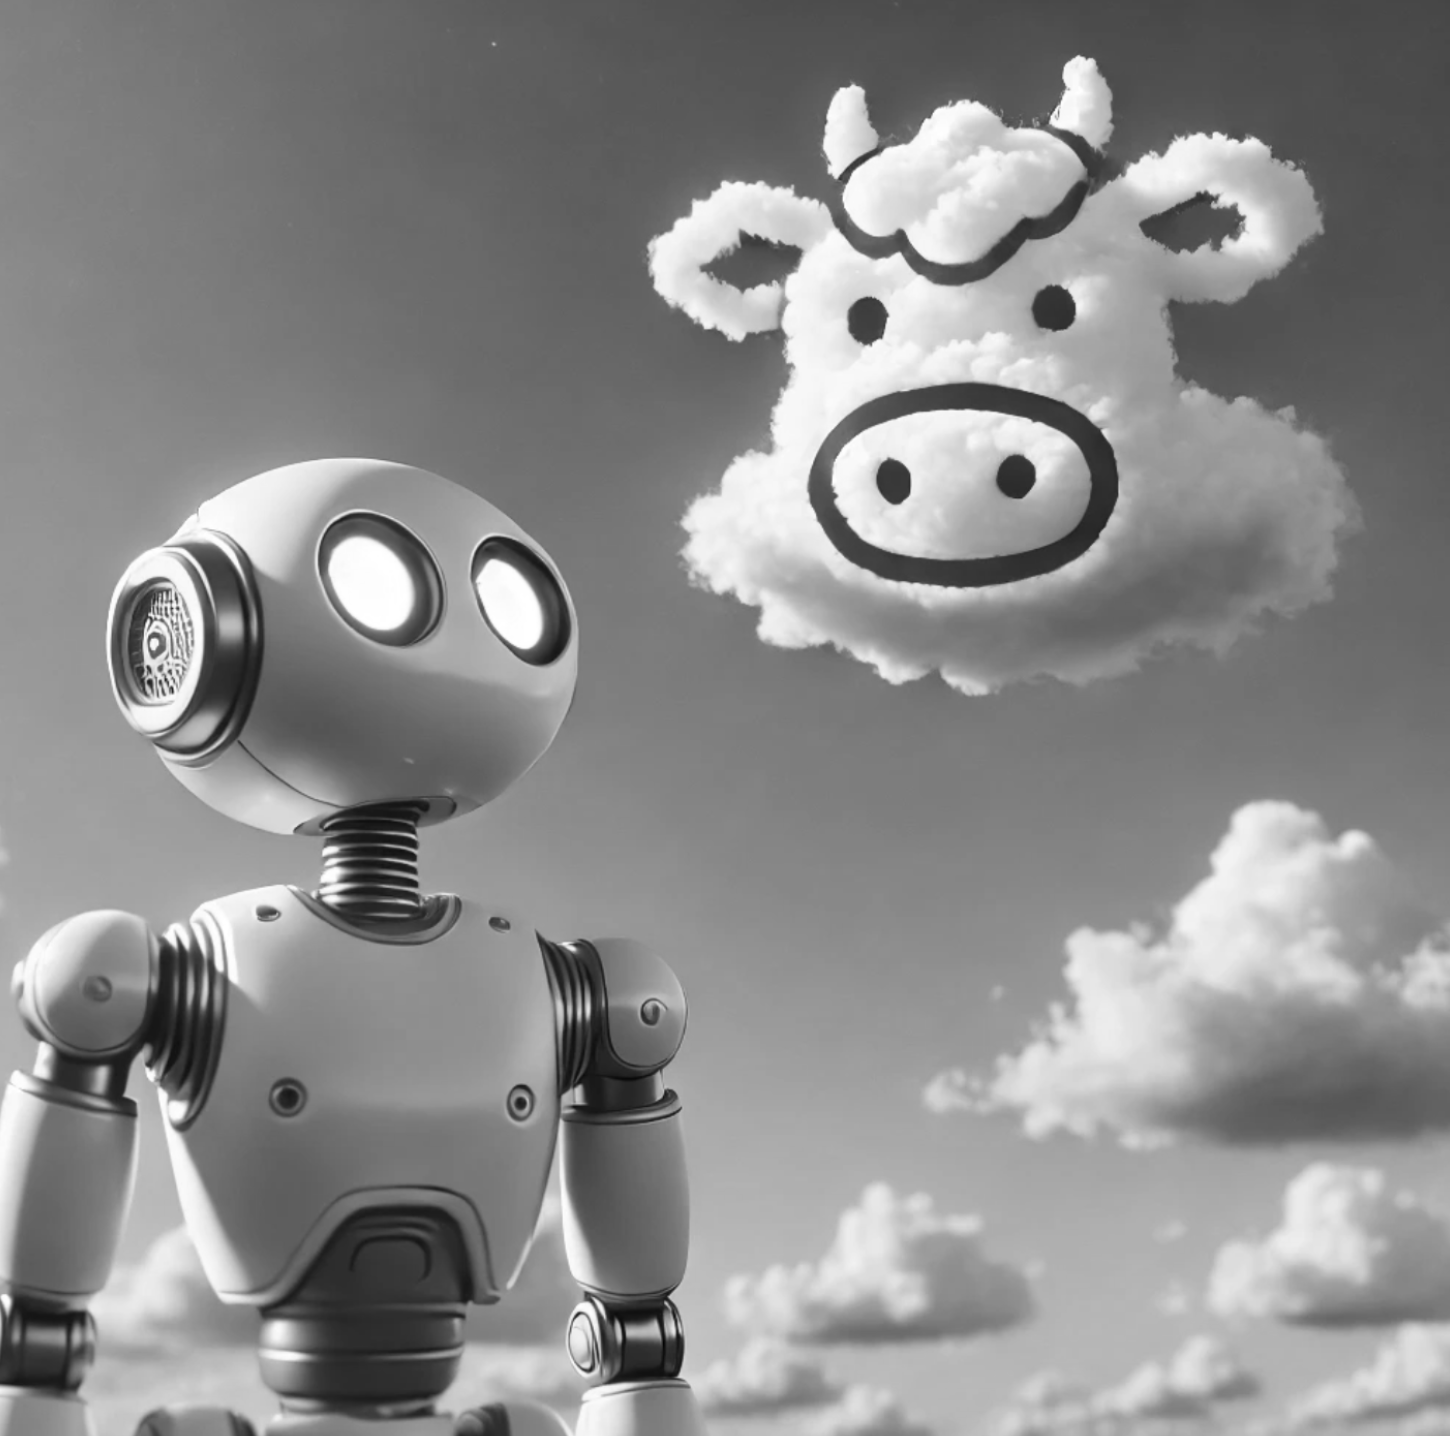
\includegraphics[height=3cm]{img/robot_emergence.png}
  \end{center}

\end{frame}





\begin{frame}{From the algorithmic agent to Bayesian inference}
Bayesian inference arises as agents strive for efficient compression, prediction and planning \cite{ruffiniNavigatingComplexityHow2024}, linking with Active Inference \cite{parr2022active}.
\begin{itemize}
    \item \textbf{Thesis}: Probability and Bayesian inference are consequences of agenthood and AIT.
    \item \textbf{Assumption}: Agents seek to \textbf{predict the world efficiently} by finding \textbf{short programs} for data (Solomonoff prior).
    \item \textbf{Agent Limitations}:
    \begin{itemize}
        \item Computational constraints (limited resources, uncomputability of $\Ko$).
        \item Partial access to data (\textit{coarse-grained} observations).
        \item \textit{Noisy} and \textit{incomplete} data.
    \end{itemize}
\end{itemize}
\vfill
    
    $\Rightarrow$  In practice, agents approximate $\Ko$ using probabilistic methods  (e.g., Huffman coding, Lempel-Ziv, ultimately Bayesian Inference).
\end{frame}


% \begin{frame}[label=ladila]{Model-building: life and intelligence}
%  \textbf{How do agents build models?} This question connects the concepts of life, intelligence, and \SEP. \vfill
 
%  Both life and intelligence represent processes to construct simple models for the persistence of algorithmic information-preserving systems across time (agents). \vfill
 
%   %Starting from {\em resilient building blocks (static persistence)},  
%   {\textbf{Life}} is an algorithmic process: program building carried not solely by the individual agent, but by the \textit{transgenerational agent} through evolution for {\em tele-homeostasis} (preservation of kind)\cite{Walker2013, Chaitin2012-wd}. \vfill

%    Evolutive pressure gives rise to the next leap, {\textbf{intelligence}}: agents that, starting from their static model (DNA in \textit{life})   build higher-level compressive models of the world within their lifetimes, e.g., using plastic brains.\vfill

%    What comes after \textit{life} and \textit{intelligence}? Symbiosis with AI?
  
% \end{frame}

 